\documentclass[../mathNotesPreamble]{subfiles}

\providecommand{\relscalefact}{1.4}
\begin{document}
\relscale{\relscalefact}
  \section{10.5: Rooted Trees}

  \begin{defn*}
    \begin{itemize}
      \item A \textbf{rooted tree} is a tree in which there is one vertex that is distinguished from the others and is called the \textbf{root}.
      \item The \textbf{level} of a vertex is the number of edges along the unique path between it and the root.
      \item The \textbf{height} of a rooted tree is the maximum level of any vertex of the tree.
      \item Given the root or any internal vertex $v$ of a rooted tree, the \textbf{children} of $v$ are all those vertices that are adjacent to $v$ and are one level farther away from the root than $v$.
      \item If $w$ is a child of $v$, then $v$ is called the \textbf{parent} of $w$, and two distinct vertices that are both children of the same parent are called \textbf{siblings}.
      \item Given two distinct vertices $v$ and $w$, if $v$ lies on the unique path between $w$ and the root, then $v$ is an \textbf{ancestor} of $w$ and $w$ is a \textbf{descendant} of $v$.
    \end{itemize}
  \end{defn*}

  \begin{center}
    \begin{tikzpicture}[
      level distance=12.5mm,
      level 1/.style={sibling distance=30mm},
      level 2/.style={sibling distance=15mm},
      level 3/.style={sibling distance=10mm},
      every node/.style={circle, fill=black, inner sep=1.5pt},
      myLabels/.style={anchor=west,fill=none, inner sep=10pt},]
      \node[label=90:$v_0$] (v0) {}
        child{node[label=180:$v_1$] (v1) {}
          child{node[label=180:$v_4$] (v4) {}
            child{node[label=-90:$v_7$] (v7) {}}
            child{node[label=-90:$v_8$] (v8) {}}
          }
          child{node[label=-90:$v_5$] (v5) {}
          }
        }
        child {node[label=0:$v_2$] (v2) {}
          child{node[label=-90:$v_6$] (v6) {}}
          child[missing]
        }
        child {node[label=-90:$v_3$] (v3) {}};

      \coordinate (labels) at ($(v0)+(45mm,0)$);
      \draw[dashed, shorten <=5mm] (v0) -- (labels|-v0) node[myLabels] {Level $0$};
      \draw[dashed, shorten <=5mm] (v3) -- (labels|-v3) node[myLabels] {Level $1$};
      \draw[dashed, shorten <=5mm] (v6) -- (labels|-v6) node[myLabels] {Level $2$};
      \draw[dashed, shorten <=5mm] (v8) -- (labels|-v8) node[myLabels] {Level $3$};
    \end{tikzpicture}
  \end{center}
  \pagebreak

  \begin{defn*}
    \begin{itemize}
      \item A \textbf{binary tree} is a rooted tree in which every parent has at most two children.
      \item Each child in a binary tree is designated either a \textbf{left child} or a \textbf{right child} (but not both), and every parent has at most one left child and one right child.
      \item A \textbf{full binary tree} is a binary tree in which each parent has exactly two children.
    \end{itemize}

    Given any parent $v$ in a binary tree $T$, if $v$ has a left child, then the \textbf{left subtree} of $v$ is the binary tree
    \begin{itemize}
      \item whose root is the left child of $v$,
      \item whose vertices consist of the left child of $v$ and all its descendants, and
      \item whose edges consist of all those edges of $T$ that connect the vertices of the left subtree.
    \end{itemize}
    The \textbf{right subtree} of $v$ is defined analogously.
  \end{defn*}

  \begin{center}
    \begin{tikzpicture}[
      level distance=12.5mm,
      level/.style={sibling distance=70mm/#1},
      every node/.style={circle, fill=black, inner sep=1.5pt},]
      \node[label=90:Root] (v0) {}
        child{node[label=135:$v_1$] (v1) {}
          child{node[label=135:$v_3$] (v3) {}
          }
          child{node[label=45:$v_4$] (v4) {}
          }
        }
        child{node[label=45:$v_2$] (v2) {}
          child{node[label=135:$v_5$] (v5) {}
            child[missing]
            child{node[label=45:$v_7$] (v7) {}
              child{node[label=135:$v_{10}$] (v10) {}
                child{node[label=-90:$v_{13}$] (v13) {}
                }
                child[missing]
              }
              child{node[label=45:$v_{11}$] (v11) {}
                child{node[label=-90:$v_{14}$] (v14) {}
                }
                child{node[label=-90:$v_{15}$] (v15) {}
                }
              }
            }
          }
          child{node[label=45:$v_6$] (v6) {}
            child{node[label=0:$v_8$] (v8) {}
            }
            child{node[label=45:$v_9$] (v9) {}
              child[missing]
              child{node[label=45:$v_{12}$] (v12) {}
                child{node[label=-90:$v_{16}$] (v16) {}
                }
                child{node[label=-90:$v_{17}$] (v17) {}
                }
              }
            }
          }
        };
    \end{tikzpicture}
  \end{center}
  \pagebreak

%  \begin{ex*}
%    %TODO algebraic expressions (p734)
%  \end{ex*}
%  \pagebreak

  \begin{thmBox*}[Theorem 10.5.1]
    If $k$ is a positive integer and $T$ is a full binary tree with $k$ internal vertices, then
    \begin{itemize}
      \item $T$ has a total of $2k+1$ vertices, and
      \item $T$ has $k+1$ leaves.
    \end{itemize}

    \textbf{Theorem 10.5.2}\newline
    For ever integer $h\geq 0$, if $T$ is any binary tree with height $h$ and $t$ leaves, then
      \[t\leq 2^h \Leftrightarrow \log_2(t)\leq h.\]

    \textbf{Corollary 10.5.3}\newline
    A full binary tree of height $h$ has $2^h$ leaves.
  \end{thmBox*}
  \begin{ex*}
    Determine if the following binary trees can exist:
    \begin{extasks}[after-item-skip=\stretch{1}](1)
      \task %Q 10.5.13
        Binary tree, height $4$, eight leaves
      \task %Q 10.5.15
        Full binary tree, nine vertices, five internal vertices
      \task %Q 10.5.16
        Full binary tree, four internal vertices
      \task %Q 10.5.18
        Full binary tree, height $4$, eighteen leaves
    \end{extasks}
    \vspace*{\stretch{1}}
  \end{ex*}
  \pagebreak

  \begin{defn*}
    \begin{itemize}
      \item A \textbf{binary search tree} is a binary tree in which data records can be stored, searched, and processed.
      \item Each element is assigned a \textbf{key}, which is used to order the elements.
    \end{itemize}
    In a binary tree, for every internal vertex $v$:
    \begin{itemize}
      \item all the keys in the left subtree of $v$ are less than the key in $v$, and
      \item all the keys in the right subtree of $v$ are greater than the key in $v$.
    \end{itemize}
  \end{defn*}
  \begin{ex*}
    The following is a binary search tree for the following keys:
      \[15, 10, 19, 25, 12, 4\]
    \begin{center}
      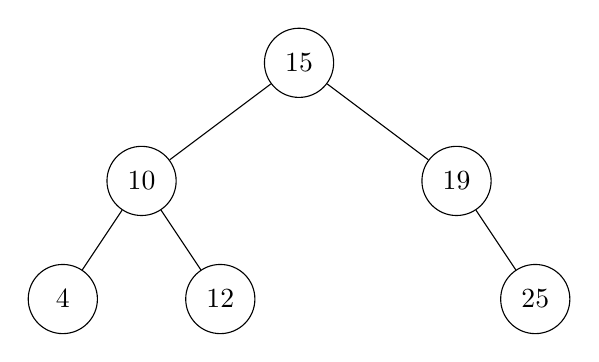
\begin{tikzpicture}[
        level distance=15mm,
        level/.style={sibling distance=40mm/#1},
        every node/.style={circle, draw=black, minimum size=25pt, inner sep=0pt},]
        \node (15) {$15$}
          child{ node (10) {$10$}
            child{ node(4) {$4$}
            }
            child{ node (12) {$12$}
            }
          }
          child{ node (19) {$19$}
            child[missing]
            child{ node (25) {$25$}
            }
          };
      \end{tikzpicture}
    \end{center}
  \end{ex*}

  \begin{ex*}
    Build the binary search tree for the keys $19, 10, 25, 4, 15, 12$
    \vspace*{\stretch{1}}
  \end{ex*}
  \pagebreak

  \begin{algorithm}[H]
    \LinesNotNumbered
    \TabPositions{40mm}
    \SetKwInOut{Input}{Input}
    \SetKwInOut{Output}{Output}
    \Input{A totally ordered, nonempty set $K$ of keys}

    Initialize $T$ to have one vertex, the root, and no edges\\
    Choose a key from $K$ to insert into the root\\
    \While{(there are still keys to be added)}{
      Choose a key, \texttt{newkey}, from $K$ to add.\\
      Let the root be called $v$, let \texttt{key($v$)} be the key at the root\\
      \texttt{success} $:=0$\\
      \While{\texttt{success} $==0$}{
        \uIf{\texttt{newkey} $<$ \texttt{key$(v)$}}{
          \eIf{$v$ has a left child}{
            $v_L:=$the left child\\
            $\mathrlap{v}\phantom{v_L}:=v_L$\\
          }{
            add a vertex $v_L$ to $T$ as the left child for $v$\\
            add an edge to $T$ to join $v$ to $v_L$\\
            insert \texttt{newkey} as the key for $v_L$\\
            \texttt{success} $:=1$
          }
        }
        \uIf{\texttt{newkey} $>$ \texttt{key$(v)$}}{
          \eIf{$v$ has a right child}{
            $v_R:=$the right child\\
            $\mathrlap{v}\phantom{v_R}:=v_R$
          }{
            add a vertex $v_R$ to $T$ as the right child for $v$\\
            add an edge to $T$ to join $v$ to $v_R$\\
            insert \texttt{newkey} as the key for $v_R$\\
            \texttt{success} $:=1$
          }
        }
      }
    }
    \Output{A binary search tree $T$ for the set $K$ of keys}
    \caption{Algorithm 10.5.1: Building a Binary Search Tree}
  \end{algorithm}
  \pagebreak
\end{document}
